\documentclass{bioinfo}
\copyrightyear{2015}
\pubyear{2015}
\usepackage[english]{babel}
\usepackage{amssymb,amsfonts,amsmath}
\usepackage{hyperref}
\usepackage{graphicx}
\usepackage{amsmath}

\newcommand{\EQ}[1]{Eq.~(\ref{eq:#1})}
\newcommand{\EQS}[2]{Eqs.~(\ref{eq:#1}) and (\ref{eq:#2})}
\newcommand{\FIG}[1]{Fig.~\ref{fig:#1}}
\newcommand{\TAB}[1]{Tab.~\ref{tab:#1}}
\newcommand{\REF}[1]{ref.~\citep{#1}}
\newcommand{\augur}{\textbf{augur}}
\newcommand{\auspice}{\textbf{auspice}}
\newcommand{\nextflu}{\textbf{nextflu}}


%%%%%%%%%%%%%%%%%%%%%%%%%%%%%%%%%%%%%%%%%%%%%%%%%%%%%%%%%%%%%%%%%%%%%%%%%%%%%%
\begin{document}
%%%%%%%%%%%%%%%%%%%%%%%%%%%%%%%%%%%%%%%%%%%%%%%%%%%%%%%%%%%%%%%%%%%%%%%%%%%%%%
\title[Tracking of seasonal influenza virus evolution]{nextflu: Real-time tracking of seasonal influenza virus evolution in humans}
\author{Richard~A.~Neher$^{1}$ and Trevor Bedford$^{2}$}
\address{$^{1}$Max Planck Institute for Developmental Biology, 72076 T\"ubingen, Germany, and $^{2}$Vaccine and Infectious Disease Division, Fred Hutchinson Cancer Research Center, Seattle, WA 98109, USA}
\history{Received on XXXXX; revised on XXXXX; accepted on XXXXX}

\editor{Associate Editor: XXXXXXX}

%\date{\today}
\maketitle

%%%%%%%%%%%%%%%%%%%%%%%%%%%%%%%%%%%%%%%%%%%%%%%%%%%%%%%%%%%%%%%%%%%%%%%%%%%%%%
\begin{abstract} \section{Summary:} Seasonal influenza viruses evolve rapidly, allowing them to evade immunity in their human hosts and reinfect previously infected individuals.
Similarly, vaccines against seasonal influenza need to be updated frequently to protect against an evolving virus population.
We have thus developed a processing pipeline and browser-based visualization that allows convenient exploration and analysis of the most recent influenza virus sequence data.
This web-application displays a phylogenetic tree that can be decorated with additional information such the viral genotype at specific sites, sampling location, and derived statistics that have been shown to be predictive of future virus dynamics.
Additionally, mutation, genotype and clade frequency trajectories are calculated and displayed.

\section{Availability and implementation:} Python and Javascript source code is freely available from \url{https://github.com/blab/nextflu}, while the web-application is live at \url{http://nextflu.org}.

\section{Contact:} tbedford@fredhutch.org

\end{abstract}
%%%%%%%%%%%%%%%%%%%%%%%%%%%%%%%%%%%%%%%%%%%%%%%%%%%%%%%%%%%%%%%%%%%%%%%%%%%%%%

%%%%%%%%%%%%%%%%%%%%%%%%%%%%%%%%%%%%%%%%%%%%%%%%%%%%%%%%%%%%%%%%%%%%%%%%%%%%%%
%\section*{Introduction}

Every year, seasonal influenza infects between 10\% and 20\% of the global population resulting in substantial human morbidity and mortality \citep{flufactsheet}.
Vaccination remains the most effective public health measure to combat seasonal epidemics.
However, influenza viruses constantly evolve and thereby undergo antigenic drift, allowing drifted viruses to reinfect those in the human population with acquired immunity to previously circulating strains.
Owing to antigenic drift, the seasonal influenza vaccine needs frequent updating to remain effective.
In any given year, the particular choice of vaccine strain plays a major role in determining vaccine efficacy and so it is of critical importance to develop tools to analyze the ongoing evolution of the influenza virus population in order to aid vaccine strain selection.
The program \nextflu{} presents a near real-time display of genetic relationships among influenza viruses and allows investigation of currently available sequence data.
Currently, \nextflu{} tracks all four circulating lineages of seasonal influenza: A/H3N2, A/H1N1pdm, B/Victoria and B/Yamagata.

\begin{figure}[t!]
	\centering
	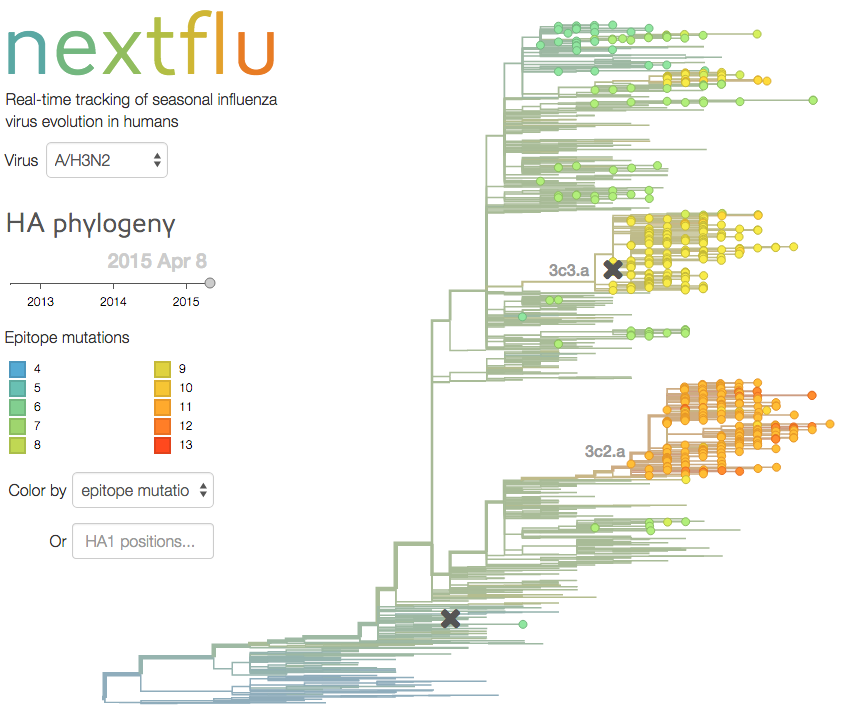
\includegraphics[width=0.99\columnwidth]{tree}
	\caption[]{The \nextflu{} website with the user interface on the left and the phylogenetic tree on the right.}
	\label{fig:tree}
\end{figure}

In implementation, \nextflu{} consists of a processing pipeline written in Python called \augur{} that analyzes virus sequence data and a JavaScript-based browser visualization called \auspice{} that displays this processed information.
As input, \augur{} requires a FASTA file of sequences with FASTA header labels containing relevant information such as the strain name, the sampling date and passage history.
For this purpose, influenza sequence data for the hemagglutinin (HA) gene is downloaded from the GISAID EpiFlu database \citep{GISAID}, which contains the most up-to-date collection of seasonal influenza viruses.
The first step in the processing pipeline is to automatically select a subset of representative viruses.
Here, viruses without complete date or geographic information, viruses passaged in eggs and sequences less than 987 bases are removed.
In addition, local outbreaks are filtered by keeping only one instance of identical sequences sampled at the same location on the same day.
Following filtering, the viruses are subsampled to achieve a more equitable temporal and geographic distribution.
For our standard display period of 3 years and 50 viruses per month, this typically results in $\sim$1800 viruses, which we align using MAFFT \citep{katoh_mafft_2013}.
Once aligned, the set of virus sequences is further cleaned by removing insertions relative to the outgroup to enforce canonical HA site numbering, by removing sequences that show either too much or too little divergence relative to the expectation given sampling date, and by removing known reassortant clusters.

From the filtered and cleaned alignment, \augur{} builds a phylogenetic tree using FastTree \citep{price_fasttree_2009}, which is then further refined using RAxML \citep{stamatakis_raxml_2014}.
Next, the state of every internal node of the tree is inferred using a marginal maximum likelihood method and missing sequence data at phylogeny tips is filled with the nearest ancestral sequence at these sites.
Internal branches without mutations are collapsed into polytomies.
The final tree is decorated with the attributes to be displayed in the browser. %, as described below.  


In addition to the phylogenetic tree, \augur{} estimates the frequency trajectories of mutations, genotypes and clades in the tree. 
Frequency trajectories are represented as a linear interpolation $x(t)$ of pivot frequencies $x_i$ at time points $t_i$ spaced one month apart. 
The frequencies $x_i$ corresponding to a feature $\phi$ (e.g.\ mutation) are estimated by simultaneously maximizing the Bernoulli observation model 
\begin{equation}
	\label{eq:obs}
	f(\mathbf{x}) = \prod_{v\in V_\phi} x(t_v) \prod_{v\notin V_{\phi}} (1-x(t_v))
\end{equation}
where $V_{\phi}$ is the set of viruses carring attribute $\phi$ and $x(t_v)$ is the sampling timepoint of virus $v$, and the process noise model
\begin{equation}
	\label{eq:freq}
	g(\mathbf{x}) = \mathrm{exp}\left(
		-\sum_i \frac{(\Delta x_i - \epsilon\Delta x_{i-1})^2}{2\gamma \Delta t_i}
	\right)
\end{equation}
where $\Delta x_i = x_i-x_{i-1}$, $\Delta t_i = t_i-t_{i-1}$, $\gamma$ parameterizes the smoothing imposed on the frequency estimate and $\epsilon$ parameterizes our expectation of frequency changes in interval $i$ based on the  change in interval $i-1$.
$\epsilon=0$ implies that frequency changes are uncorrelated from one interval to the next, while $\epsilon=1$ implies that the most likely $\Delta x_i$ is $\Delta x_{i-1}$.
We typically use $\epsilon = 0.7$.
Here, the objective function $\mathrm{log}(f) + \mathrm{log}(g)$ is maximized using SciPy's implementation of a downhill simplex algorithm \citep{oliphant_python_2007}.
To speed up convergence, optimization is first done using a coarse grid of pivot points which is subsequently refined to 12 pivots per year. Frequency estimation is done for mutations, particular genotypes, and major clades of the tree.
At the end of the \augur{} pipeline, JSON files are exported containing the annotated phylogenetic tree, sequence data and frequency trajectories.

These JSON files are then visualized by \auspice{} using D$^3$ \citep{bostock_d3_2011} and the phylogenetic tree displayed (\FIG{tree}).
The user can explore the data interactively by selecting viruses from different dates or by coloring the tree by attributes such as:
\begin{itemize}
	\item \textit{epitope mutations} at sites generally associated with antibody binding have been suggested to be predictive of future clade success \citep{luksza_predictive_2014},
%	\item non-epitope mutations: 
%	Mutations outside epitopes tend to be damaging and anti-correlated with clade expansion \citep{luksza_predictive_2014}.
    \item \textit{receptor binding mutations} at seven positions close to the receptor binding site have been shown to be responsible for major antigenic transitions in the past decades \citep{koel_substitutions_2013},
    \item \textit{local branching index} is the exponentially weighted tree length surrounding a node, which is associated with rapid branching and expansion of clades \citep{neher_predicting_2014},
 %   \item geographic location
    \item \textit{HA genotype} directly colors the tree by genotype at specific amino acid positions.
\end{itemize}

\begin{figure}[t]
	\centering
	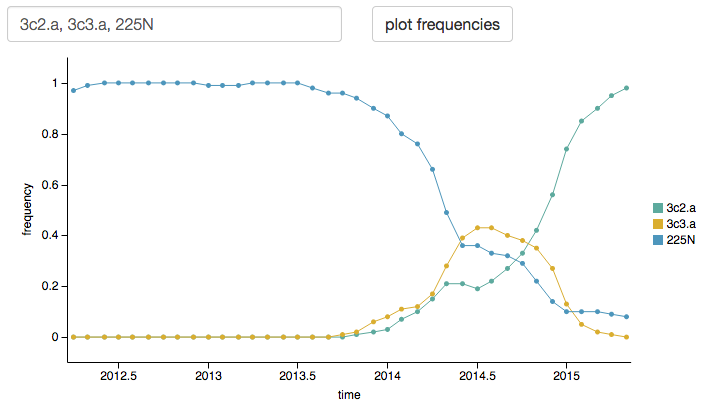
\includegraphics[width=0.99\columnwidth]{frequencies}
	\caption[]{The frequency diagram allows geography-specific plotting of frequencies of individual mutations, pairs of mutations and clades in the tree.}
	\label{fig:freq}
\end{figure}

The frequency plot below the tree (\FIG{freq}) displays the frequency trajectory of clades in the tree whenever the mouse hovers above the branch defining the clade. 
Furthermore, trajectories of individual mutations, combinations of two mutations, and predefined clades such as 3c3.a can be plotted.

%\section{Conclusion}
We built \nextflu{} to facilitate the analysis and exploration of seasonal influenza sequence data collected by laboratories around to world.
By using the most recent data and integrating phylogenies with frequency trajectories and predictors of successful clades, we hope that \nextflu{} can inform the choice of strains used in seasonal influenza vaccines. 
\nextflu{} was designed to be readily adapted to other rapidly evolving viruses and we see significant room for future developments in this area.
 
\paragraph{Funding\textcolon}This work is supported by the ERC though Stg-260686 and by the NIH through U54 GM111274.

%%%%%%%%%%%%%%%%%%%%%%%%%%%%%%%%%%%%%%%%%%%%%%%%%%%%%%%%%%%%%%%%%%%%%%%%%%%%%%
\begin{thebibliography}{}

\bibitem[Bogner {\em et~al.}, 2006]{GISAID}
Bogner,P. {\em et~al.} (2006{\em{}}) A global
  initiative on sharing avian flu data.
\newblock {\em Nature, } {\bf 442} (7106), 981--981.

\bibitem[Bostock {\em et~al.}, 2011]{bostock_d3_2011}
Bostock,M. {\em et~al.} (2011{\em{}}) D$^3$: data-driven
  documents.
\newblock {\em IEEE Trans Vis Comput Graphics, } {\bf 17} (12), 2301--2309.

\bibitem[Katoh and Standley, 2013]{katoh_mafft_2013}
Katoh,K. and Standley,D.M. (2013{\em{}}) {MAFFT} multiple sequence alignment
  software version 7: improvements in performance and usability.
\newblock {\em Mol Biol Evol, } {\bf 30}, 772--780.

\bibitem[Koel {\em et~al.}, 2013]{koel_substitutions_2013}
Koel,B.F. {\em et~al.} (2013{\em{}})
  Substitutions near the receptor binding site determine major antigenic change
  during influenza virus evolution.
\newblock {\em Science, } {\bf 342} (6161), 976--979.

\bibitem[\L{}uksza and L\"a{}ssig, 2014]{luksza_predictive_2014}
\L{}uksza,M. and L\"a{}ssig,M. (2014{\em{}}) A predictive fitness model for
  influenza.
\newblock {\em Nature, } {\bf 507} (7490), 57--61.

\bibitem[Neher {\em et~al.}, 2014]{neher_predicting_2014}
Neher,R.A. {\em et~al.} (2014{\em{}}) Predicting evolution
  from the shape of genealogical trees.
\newblock {\em eLife Sciences, } {\bf 3}, e03568.

\bibitem[Oliphant, 2007]{oliphant_python_2007}
Oliphant,T. (2007{\em{}}) Python for scientific computing.
\newblock {\em Comput Sci Eng, } {\bf 9} (3), 10--20.

\bibitem[Price {\em et~al.}, 2009]{price_fasttree_2009}
Price,M.N. {\em et~al.} (2009{\em{}}) {FastTree:} computing
  large minimum evolution trees with profiles instead of a distance matrix.
\newblock {\em Mol Biol Evol, } {\bf 26} (7), 1641--50.

\bibitem[Stamatakis, 2014]{stamatakis_raxml_2014}
Stamatakis,A. (2014{\em{}}) {RAxML} version 8: a tool for phylogenetic analysis
  and post-analysis of large phylogenies.
\newblock {\em Bioinformatics, } {\bf 30} (9), 1312--1313.

\bibitem[{World Health Organization}, 2009]{flufactsheet}
{World Health Organization} (2009{\em{}}) {\em {Influenza Fact sheet}}.
\newblock Available at http://www.who.int/mediacentre/factsheets/fs211/en/.

\end{thebibliography}
%%%%%%%%%%%%%%%%%%%%%%%%%%%%%%%%%%%%%%%%%%%%%%%%%%%%%%%%%%%%%%%%%%%%%%%%%%%%%%
\end{document}
%%%%%%%%%%%%%%%%%%%%%%%%%%%%%%%%%%%%%%%%%%%%%%%%%%%%%%%%%%%%%%%%%%%%%%%%%%%%%%
